This chapter presents the design of a safe controller for the  robotic patient manipulator in 3D Cartesian space, where the unsafe region is defined as an ellipsoid with static boundaries, i.e. fixed in space with respect to time. The unsafe region is defined such that it is within the reach of the instrument tip. 

The robotic patient manipulator constitutes four "arms" (see \autoref{fig:master-slave_surgery}) each comprising a number of arm links, whose joints are fixed by electromagnets that are manually released for positioning of these links; followed by the robot "hand" and instrument links, whose joints are available for automated control on the modified AAU da Vinci robot. Only the controllable part of the robotic patient manipulator, as displayed in \autoref{fig:robot_hand_3d}, is considered in the design of the 3D Cartesian space controller. 

\begin{figure}[htbp]
\centering
\subbottom[Robotic patient manipulator.]{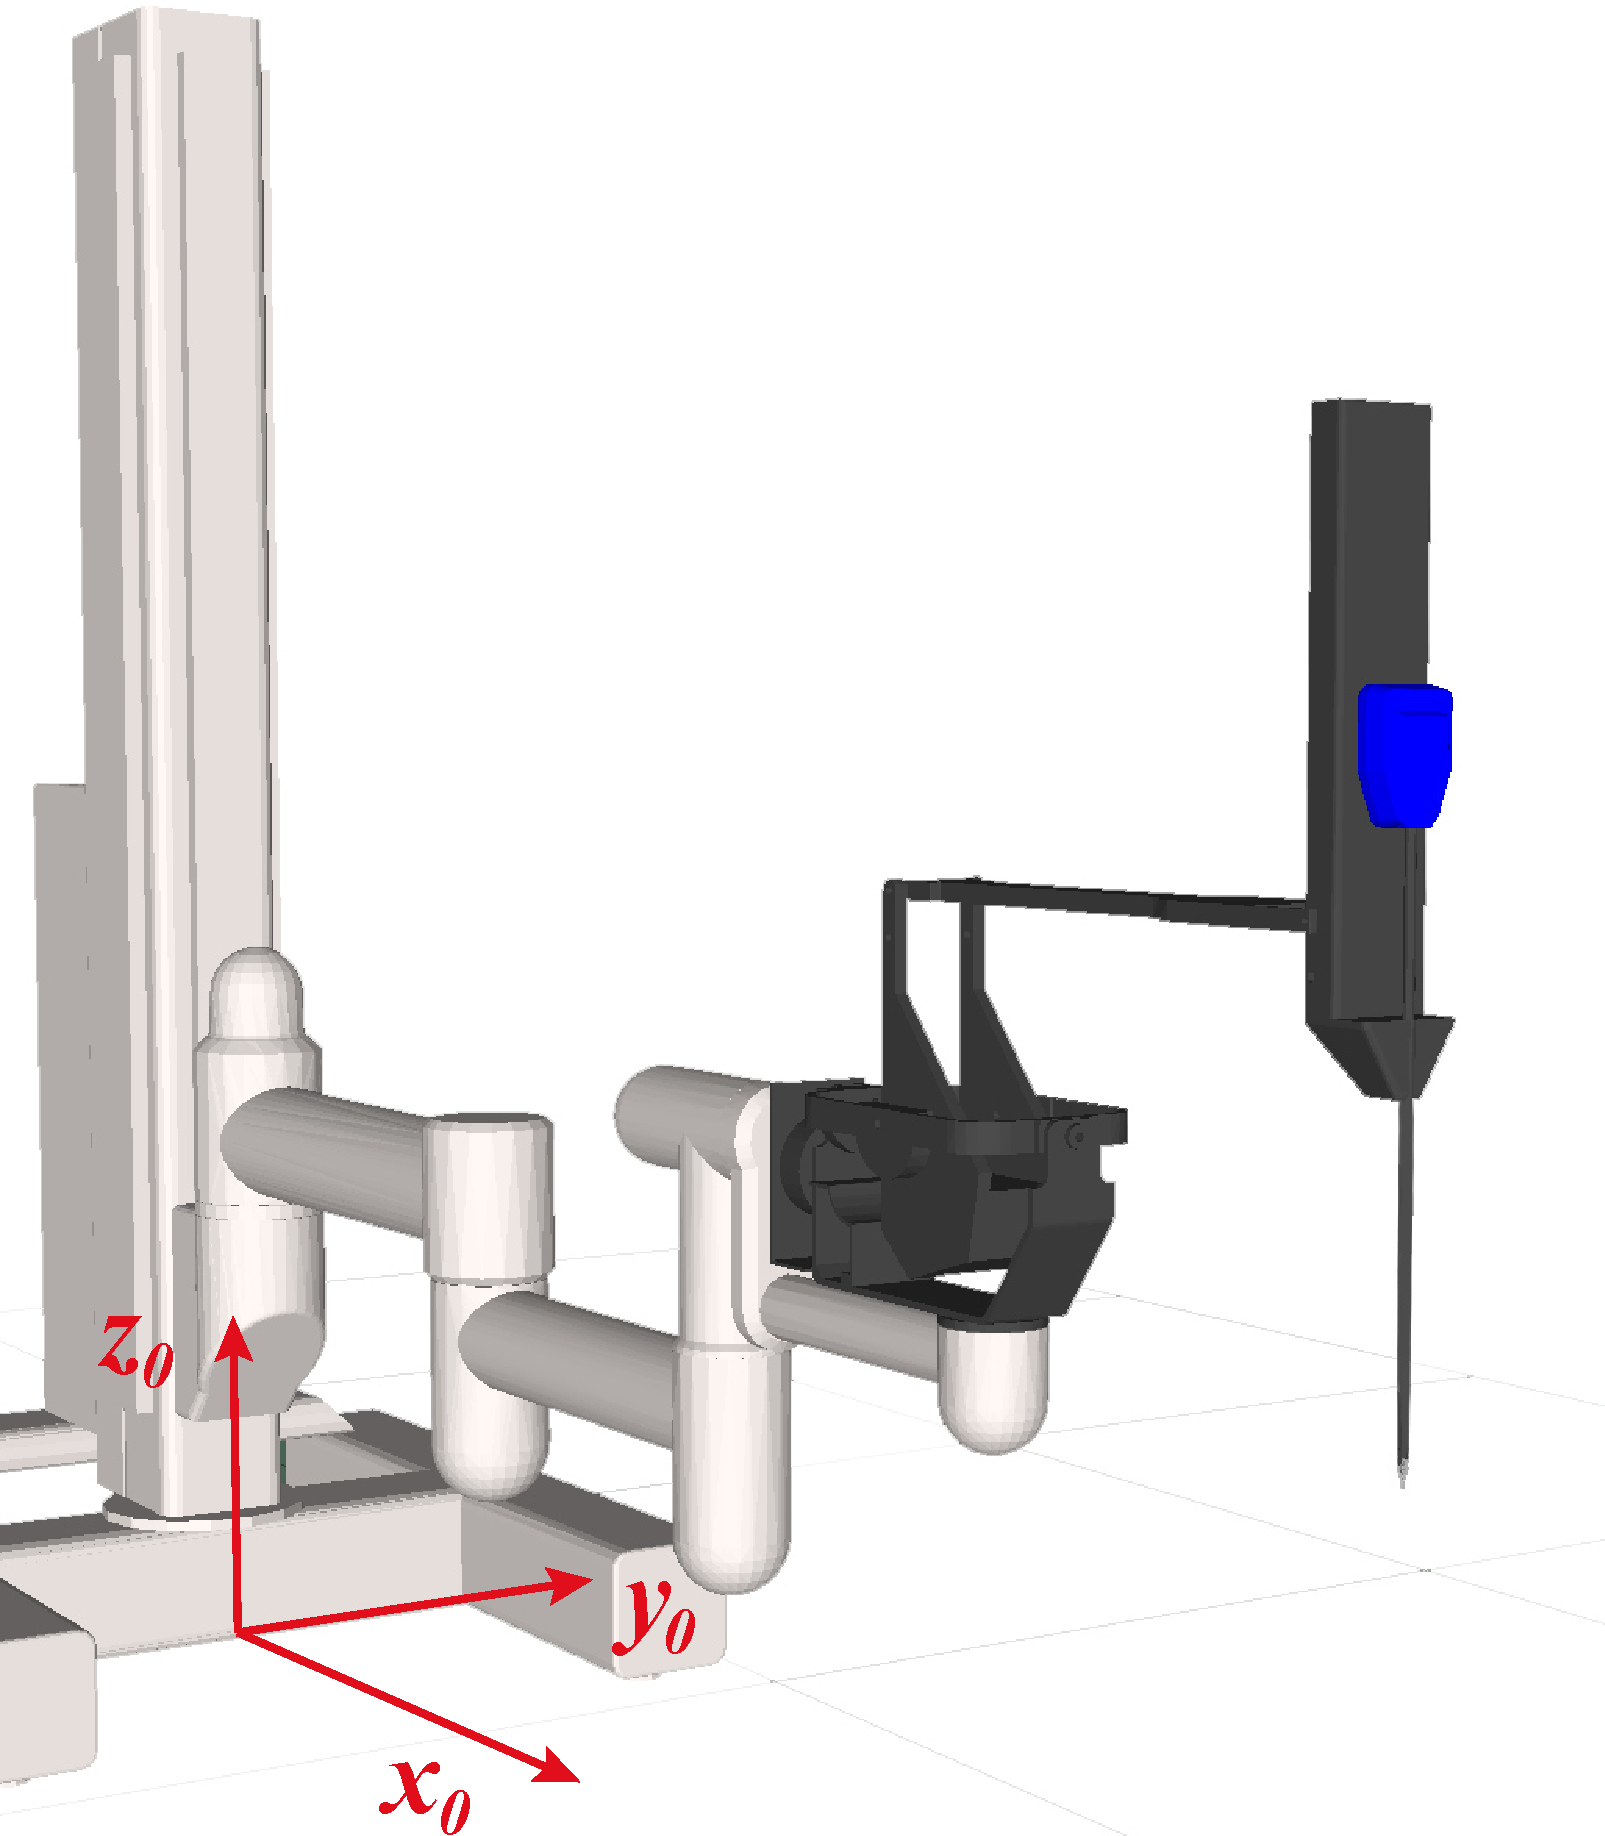
\includegraphics[width=0.45\textwidth]{rviz_09_17_18_frame1.pdf}\label{fig:rviz_09_17_18_frame}}%
	\hspace*{5mm}
\subbottom[Robotic "hand" and instrument.]{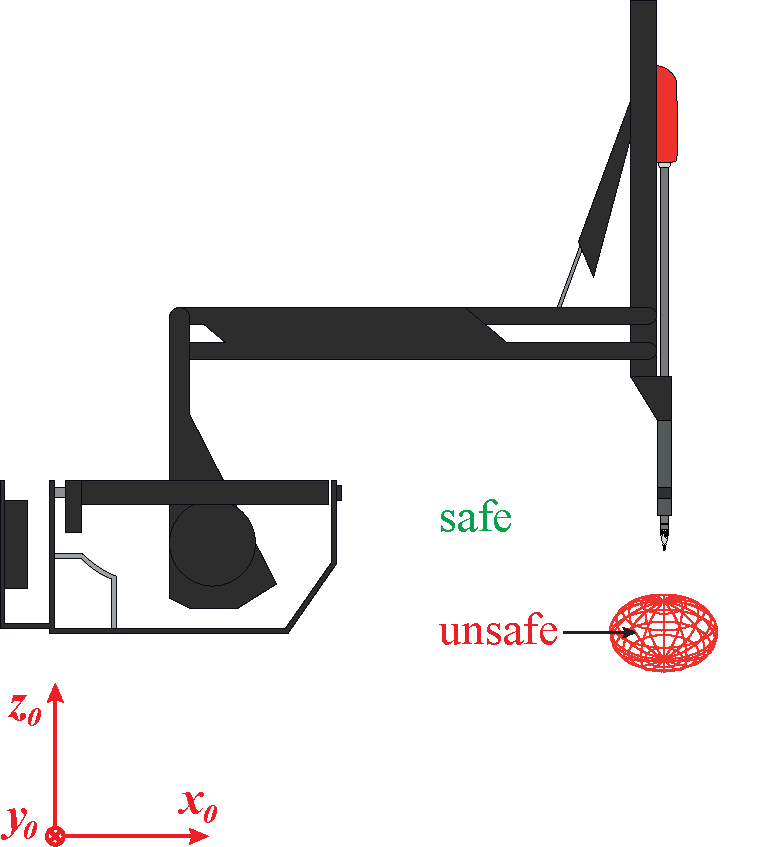
\includegraphics[width=0.45\textwidth]{robot_hand_unsafe_region.pdf}\label{fig:robot_hand_unsafe_region}}%
\caption{Patient manipulator and a fixed region within the reachable space $\mathcal{X}$ that is unsafe, $\mathcal{X}_u$, marked by a red ellipsoid.}
\label{fig:robot_hand_3d}
\end{figure}

The controller is designed for and tested on the da Vinci robot comprising the prismatic slide joint as described in \autoref{chap:cbf_1d_static} as well as five independent revolute joints. In order to design a controller in 3D Cartesian space for the robot, a kinematic description of the robot links and joints is necessary as a translation between the 3D Cartesian space and the 6D joint space.
Hence, before modelling the system and designing a controller, the kinematics of the AAU da Vinci robot is presented in the following section along with considerations for the definition of the coordinate frames and the transformation between them constituting the kinematic description of the robot.


\section{Kinematics of the AAU da Vinci Robot}
A kinematic description of an object requires defining a right-handed coordinate frame fixed in the object and a coordinate frame fixed in inertial space, the latter which the position and orientation of the object can be described relative to. This relative orientation and position of an object (or the frame $i$ fixed in it) with respect to another frame $j=i-1$ can be described through a transformation matrix $T$, containing the orthonormal rotation matrix $R$ and the translation vector $p$ of the frame origin, as 
\begin{equation}
^j_iT = 
\begin{bmatrix}
^j_iR & ^j_ip\\
0 & 1
\end{bmatrix}, \label{eq:kin_transformation}
\qquad \text{where} \qquad
^j_ip = 
\begin{bmatrix}
a\\b\\d
\end{bmatrix}
\end{equation}
and the simplest rotation matrices $R$ are rotations about a single axis, which can be combined to obtain an arbitrary rotation
\begin{small}
	\begin{equation}
	R_x(\alpha) = 
	\begin{bmatrix}
	1 & 0 & 0\\
	0 & \cos\alpha & -\sin\alpha\\
	0 & \sin\alpha & \cos\alpha
	\end{bmatrix} 
	\qquad
	R_y(\beta) = 
	\begin{bmatrix}
	\cos\beta & 0 & \sin\beta \\
	0 & 1 & 0\\
	-\sin\beta & 0 & \cos\beta
	\end{bmatrix}
	\qquad
	R_z(\theta) = 
	\begin{bmatrix}
	\cos\theta & -\sin\theta & 0\\
	\sin\theta & \cos\theta & 0\\
	0 & 0 & 1
	\end{bmatrix}
	\label{eq:RxRyRz_chapter}
	\end{equation}
\end{small}

For the robotic patient manipulator comprising a number of links, coordinate frames are defined for each degree of freedom, i.e. placed in each joint such that one of the frame axes is the axis of free rotation or translation. The kinematic chain is now the sequence of alternate links and joints starting from the link fixed in inertial space and ending at the tip of the robotic tool. The link preceding a joint is its parent link, while the link succeeding it is its child link. The transformation between any two frames is given as the product of the transformation matrices in the kinematic chain between them. An example of a sequence of transformations can be seen in \autoref{app:kinematic_model_robot}.

For the resolution of frame definitions it is preferred to adapt the  robot coordinate frame convention \gls{dh} because it is one of the most widespread kinematic descriptions in the robot kinematics community, and because it describes transformations between two successive frames in the kinematic chain on a succinct and standardized form
\begin{equation}
\hspace*{-2mm}
\small
^{i-1}_{\phantom{-1}i} T =
\begin{bmatrix}
R_z(\theta_i) & \begin{bmatrix}0\\ 0\\ d_i\end{bmatrix}\\
0 & 1
\end{bmatrix}
\begin{bmatrix}
R_x(\alpha_i) & \begin{bmatrix}a_i\\ 0\\ 0\end{bmatrix}\\
0 & 1
\end{bmatrix}
\label{eq:dh}
\end{equation}
In the \gls{dh} kinematic description each frame is fixed with respect to its parent link, and its $z$-axis is aligned with the actuation axis of its child link. The free rotation/translation always taking place around/along the local $z$ axis, and as seen from \autoref{eq:dh} any fixed or free rotation/translation about/along the $z$-axis is implemented (intrinsically) before any fixed rotation/translation about/along the (new) $x$-axis. For more details on the \gls{dh} convention and robot frames defined according to is, see \autoref{sec:denavit_hartenberg}.

%\begin{itemize}
%	\itemsep-1.3mm 
%	\item variable/parameter $\theta_i$ is the angle from $x_{i-1}$ to $x_i$ about $z_{i-1}$
%	\item variable/parameter $d_i$ is the distance from origin $i-1$ to $x_i$ measured along $z_{i-1}$
%	\item parameter $a_i$ is the distance from $z_{i-1}$ to $z_i$ measured along $x_i$
%	\item parameter $\alpha_i$ is the angle from $z_{i-1}$ to $z_i$ about $x_i$
%\end{itemize}

In the robot description in \gls{ros}, however, the kinematics are described in the \texttt{xacro} files on the form
\begin{equation}
\hspace*{-2mm}
\small
^{i-1}_{\phantom{-1}i}T =
\begin{bmatrix}
R_z(\text{yaw})R_y(\text{pitch})R_x(\text{roll}) & \begin{bmatrix}a_i\\ b_i\\ d_i\end{bmatrix}\\
0 & 1
\end{bmatrix}
\begin{bmatrix}
R_z(\theta_i^*)R_y(\beta_i^*)R_x(\alpha_i^*) & \begin{bmatrix}a_i^*\\ b_i^*\\ d_i^* \end{bmatrix}\\
0 & 1
\end{bmatrix}
\label{eq:xacro_transformation_chapter}
\end{equation}
Here fixed translations are implemented first, then RPY rotations (extrinsic roll (about $x$-axis), pitch (about $y$-axis), yaw (about $z$-axis) rotation), and finally the free rotation or translation (denoted by $^*$ in \autoref{eq:xacro_transformation_chapter}) about/along one of the rotated axes. Furthermore, the convention here is that each frame (joint) is fixed in its child link (corresponding to the fixed rotations preceding the free rotation), and not in its parent link as in the DH convention. The transformation  $^{i-1}_{\phantom{-1}i} T$ is implemented in joint $i$ in the \texttt{xacro} file  as (for joint 8)
\begin{lstlisting}[language=xml]
<joint name="p4_hand_pitch"  type="revolute">
<origin
xyz="0 0 0"
rpy="1.5708 0 0" />
<parent link="rcm_vitual0" />
<child link="rcm_vitual1" />
<axis xyz="0 0 1" />
...
</joint>
\end{lstlisting}

A compromise is made, defining a new set of frames for the da Vinci kinematics, adhering to the \gls{dh} constraint that each free rotation/translation is about/along the local $z$-axis. The new kinematic frames are visualized in \autoref{fig:p4_hand_compromise_frames_chapter}, the parameters listed in table \ref{tab:new_kin_short}. Furthermore, for simplification of the inverse kinematics solver, the two passive joints mimicking the hand pitch movement are removed from the existing kinematic chain, visualized in \autoref{fig:p4_hand_xacro_frames_chapter}, and parameters listed in table \ref{tab:old_kin_short} for comparison.  



\begin{table}[htbp]
	\small
	\centering
\subbottom[Old robot hand kinematics including mimicking joints, corresponding to \autoref{fig:p4_hand_xacro_frames_chapter}.]{%
	\begin{tabular}{r | rrr | ccc | c l}\hline
		& \multicolumn{3}{c|}{fixed translation  [m]} & \multicolumn{3}{c|}{fixed rotation [rad]} & freedom & \\
		frame  & $a$ ($x$)  & $b$ ($y$)  & $d$ ($z$)  & roll  & pitch & yaw & $\alpha^*, \beta^*, \theta^*$ or $d^*$ & joint name\\\hline
		7 & -0.042 & 0 & 0.161 & 0 & 0 & 0 & $\phantom{-}\alpha_7^*$ & \texttt{hand\_roll} \\
		8 & 0 & 0 & 0 & 0 & -0.288 & 0 & $-\beta_8^*$ & \texttt{hand\_pitch} \\
		9 & 0.011 & 0 & 0.186 & $\pi$ & 0.288 & 0 & $\phantom{-}\beta_8$ & mimic \texttt{hand\_pitch} \\
		10 & 0.520 & 0 & 0 & $\pi$ & 0& 0 &  $-\beta_8$ & mimic \texttt{hand\_pitch} \\
		11 & 0 & 0 & -0.120  & 0 & 0 & 0 & $\phantom{-}d_{11}^*$ & \texttt{instrument\_slide} \\
		12 & 0.052 & 0 & 0 & $\pi$ & 0 & $\pi/2$ & $\phantom{-}\theta_{12}^*$ & \texttt{instrument\_roll} \\
		13 & 0 & 0 & 0.177 & 0 & 0 & 0 & $-\alpha_{13}^*$ & \texttt{instrument\_pitch} \\
		14L & 0 & 0 & 0.009 & $\pi/2$ & $\pi/2$ & 0 & $-\theta_{14L}^*$ & \texttt{instrument\_jaw\_left} \\
		14R & 0 & 0 & 0.009 & $\pi/2$ & $\pi/2$ & 0 & $\phantom{-}\theta_{14R}^*$ & \texttt{instrument\_jaw\_right} \\
	\end{tabular}\label{tab:old_kin_short}}
	\vspace*{1mm}
\subbottom[New robot hand kinematics excluding mimicking joints, corresponding to \autoref{fig:p4_hand_compromise_frames_chapter}.]{%
	\begin{tabular}{r | rrr | ccc | c l}\hline
		& \multicolumn{3}{c|}{fixed translation  [m]} & \multicolumn{3}{c|}{fixed rotation [rad]} & freedom & \\
		frame  & $a$ ($x$)  & $b$ ($y$)  & $d$ ($z$)  & roll  & pitch & yaw & $\theta^*$ or $d^*$ & joint name\\\hline
		7 & 0.482 & 0 & 0.047 & 0 & $\pi/2$ & 0 & $\theta_7^*$ & \texttt{hand\_roll} \\
		8 & 0 & 0 & 0 & $\pi/2$ & 0 & 0 & $\theta_8^*$ & \texttt{hand\_pitch} \\
		9 & 0.097 & 0 & 0 & 0 & $-\pi/2$ &  0 & $d_9^*$ & \texttt{instrument\_slide} \\
		10 & 0 & 0 & 0 & 0 & 0 & 0 & $\theta_{10}^*$ & \texttt{instrument\_roll} \\
		11 & 0 & 0 & 0 & 0 & $\pi/2$ & 0 & $\theta_{11}^*$ & \texttt{instrument\_pitch} \\
		12L & 0.009 & 0 & 0 & $-\pi/2$ & 0 & 0 & $\theta_{12L}^*$ & \texttt{instrument\_jaw\_left} \\
		12R & 0.009 & 0 & 0 & $-\pi/2$ & 0 & 0 & $\theta_{12R}^*$ & \texttt{instrument\_jaw\_right} \\
		\end{tabular}\label{tab:new_kin_short}}
	\caption{Parameters and variables (marked with $^*$) for the robot kinematic description implemented in \gls{ros} and visualized in \autoref{fig:robot_hand_kinematics}. Free angles are named with $\alpha$ being a rotation about the $+x$-axis, $\beta$ about the $+y$-axis and $\theta$ about the $+z$-axis.}
	\label{tab:xacro_param_short}
\end{table}



\begin{figure}[htbp]
\hspace*{-15mm}
\begin{minipage}{1.15\textwidth}
	\subbottom[Old robot hand kinematics including mimick joints, parameters given in table \ref{tab:old_kin_short}.]{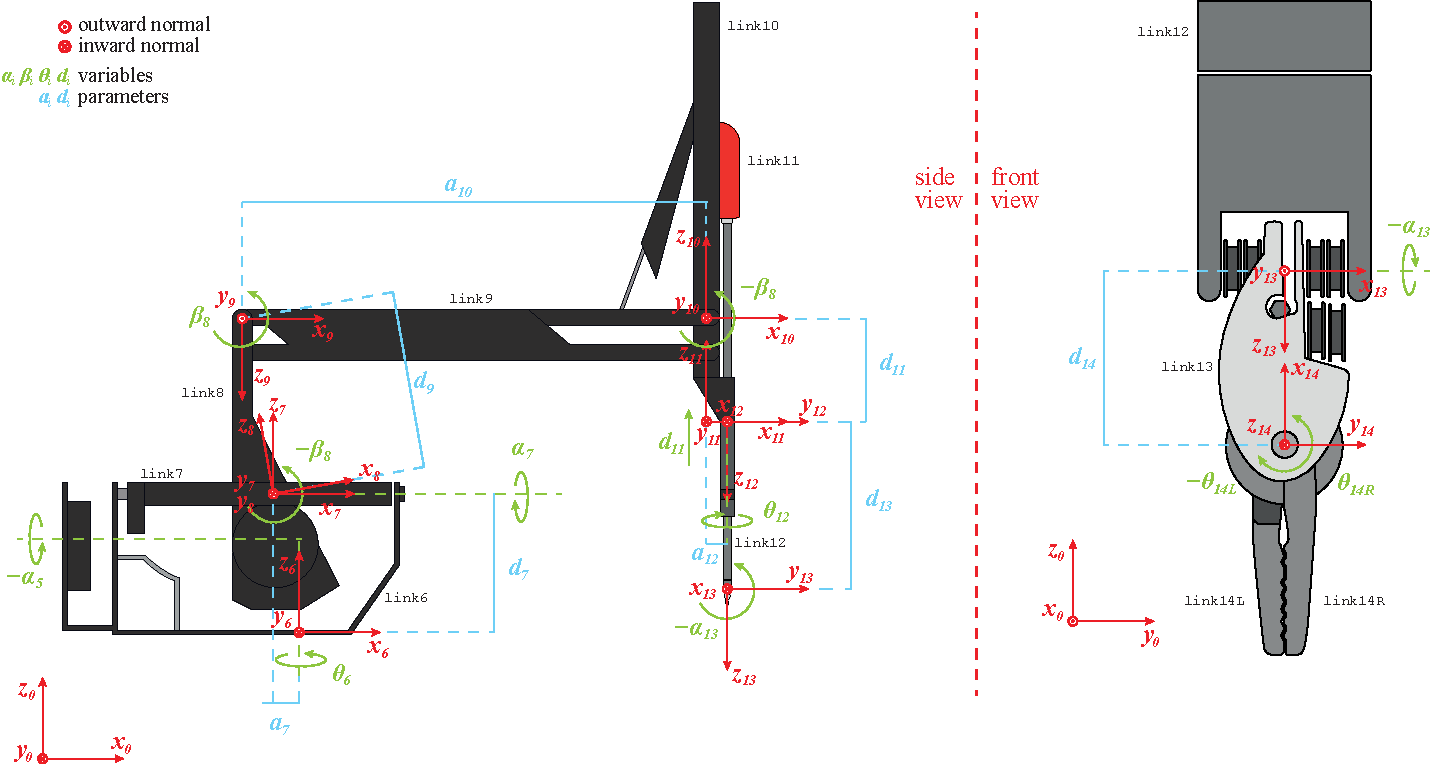
\includegraphics[width=\textwidth]{p4_hand_xacro_frames_chapter.pdf}\label{fig:p4_hand_xacro_frames_chapter}}%
	\vspace*{5mm}
	\subbottom[New robot hand kinematics excluding mimick joints, parameters given in table \ref{tab:new_kin_short}.]{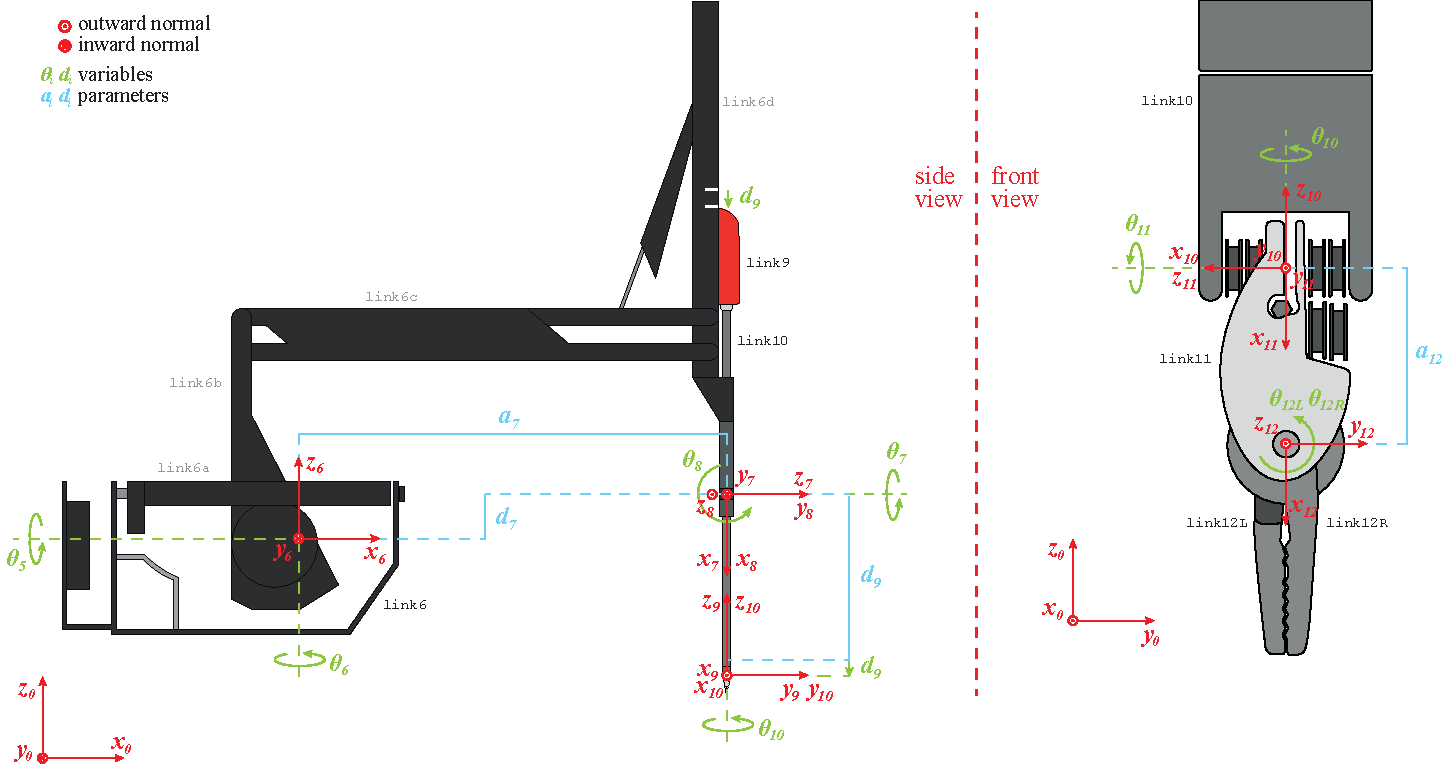
\includegraphics[width=\textwidth]{p4_hand_compromise_frames_chapter.pdf}\label{fig:p4_hand_compromise_frames_chapter}}%
	\caption{Orientation and position of coordinate frames $\Psi_7$, $\Psi_8$, etc. corresponding to the controllable joints of the robotic patient manipulator.  For convenience of placing the hand roll and pitch frames in the pivot point in the new kinematic description in \autoref{fig:p4_hand_compromise_frames_chapter}, a virtual link is inserted in the \texttt{xacro} file after each of these two joints.}
	\label{fig:robot_hand_kinematics}
\end{minipage}
\end{figure}


For more details on the old and new kinematic descriptions implemented in \gls{ros}; including all measurements of parameters, gearing ratios, code for testing the kinematic description in Matlab, and measurements of distances for different configurations; please refer to \autoref{sec:existing_kinematics} and \ref{sec:app_activejoints_kinematics} in \autoref{app:kinematic_model_robot}.










\subsection{Employing Inverse Kinematics for a Controller in 3D Cartesian Space}
The controller presented in this chapter is developed for 3D position and orientation control of the tool tip, and hence relies on the use of inverse kinematics for the (ambiguous) mapping from 3D Cartesian space to 6D joint space. The inverse of the kinematic transformation matrix presented in \autoref{eq:kin_transformation} is
\begin{equation}
^j_iT^{-1} = 
\begin{bmatrix}
^j_iR^T & -^j_iR^T\,\,^j_ip\\
0 & 1
\end{bmatrix}
\end{equation}
With the sequence of transformations from frame $k$ to frame $i$ being represented by the transformation matrix $^k_i T$, the inverse transformation, from frame $i$ to frame $k$, is then its matrix inverse $^k_i T^{-1}$
\begin{equation}
^k_iT = ^k_jT \,\, ^j_iT =
\begin{bmatrix}
^k_jR \,\, ^j_iR & ^k_jp+^k_jR \,\, ^j_ip\\
0 & 1
\end{bmatrix}
\qquad \Leftrightarrow \qquad
^k_iT^{-1} = 
\begin{bmatrix}
^j_iR^T\,\, ^k_jR^T & -\,^j_iR^T\,\, ^k_jR^T\,\,^k_jp -\, ^j_iR^T\,\, ^j_ip\\
0 & 1
\end{bmatrix}
\end{equation}
A mapping from six to three degrees of freedom is a surjective map, i.e. several elements in the 6D domain may map to the same element in the 3D co-domain. However the inverse map from 3D to 6D is neither injective nor surjective, as each element in the 3D domain can map to several elements in the 6D co-domain, and hence the mapping requires a decision of the "best" map.

In practice this mapping from the desired 3D Cartesian space configuration to a prudent 6D joint space position of the da Vinci robotic patient manipulator is handled by the \gls{kdl} inverse kinematics solver. Then the transformed joint position commands are passed to the low level controllers (see \autoref{fig:overview}).

The \gls{ik} \gls{kdl} solver employed in \gls{ros} utilizes the kinematic chain from the URDF, which is generated from the \texttt{xacro} link and joint kinematic description as presented in %\autoref{app:kinematic_model_robot}, the model implemented in ROS defined in
\autoref{sec:app_activejoints_kinematics}. From this chain (\texttt{my\_chain} in the below example) a \gls{fk} position solver is created along with an \gls{ik} velocity solver in order to define the \gls{ik} position solver:

\begin{lstlisting}[language=xml]
//Create solver based on kinematic chain
KDL::ChainFkSolverPos_recursive fksolver(my_chain);
KDL::ChainIkSolverVel_pinv iksolverv(my_chain);
KDL::ChainIkSolverPos_NR iksolver = KDL::ChainIkSolverPos_NR(my_chain,fksolver,iksolverv,100,1e-6);

KDL::JntArray q(my_chain.getNrOfJoints());
KDL::JntArray q_init(my_chain.getNrOfJoints());

//Set destination frame
double x, y, z;
std::cout << "Set end-effector position <x y z>:" << std::endl;
std::cin >> x >> y >> z;
KDL::Vector dest_pos(x,y,z);
KDL::Frame dest_frame(dest_pos);

// Compute!
int ret = iksolver.CartToJnt(q_init,dest_frame,q);
\end{lstlisting}

The \gls{kdl} \gls{ik} position solver uses the Newton-Raphson iterative numerical technique through the function \texttt{CartToJnt} to determine a prudent joint configuration implementing the desired Cartesian configuration (given as \texttt{dest\_frame} in the above example). In the above example the initial guess \texttt{q\_init} of the joint configuration is the current joint configuration, and hence care should be taken to only command small changes in configuration for the sake of fast convergence of the \gls{ik} solution.


Three dimensional positions of the tool tip is described in a frame oriented as the inertial frame and offset such that a robot configuration with all free angles and slide set to zero equals a position of the tool tip in [0,0,0].




\section{Modelling of Robot Hand Movement}
\textcolor{red}{Make measurement of step for cases: x-axis, y-axis, z-axis, and xyz at the same time. Compare to slide measurement.}

\section{Safe Controller Design for First Order System}
For simplicity, a completely decoupled system is assumed with the same characteristics for each axis as described in \autoref{subsec:model_1d}. \textcolor{red}{Argue why, something about measurement, as movements are composed from changing joint angles obviously the axes are coupled, but it is also dependent on the low level controllers on the FPGA.} Based on this, identical linear position controllers as in \autoref{eq:utilde} are used for each axis, calculated as presented in \autoref{sec:K_Nbar_1D_1storder}, which results in the closed-loop system on the safe region $\mathcal{X}_0$ on the form
\begin{equation}\label{eq:3D_sys_static}
\small
\dot{\begin{bmatrix}
	x\\y\\z
	\end{bmatrix}} =
\underbrace{\begin{bmatrix}
	-1/\tau & 0 & 0\\0 & -1/\tau & 0 \\ 0 & 0 & -1/\tau
	\end{bmatrix}
	\begin{bmatrix}
	x\\y\\z
	\end{bmatrix}}_{f(x)} +
\underbrace{\begin{bmatrix}
	1/\tau& 0 & 0 \\ 0& 1/\tau & 0 \\0& 0& 1/\tau
	\end{bmatrix}}_{g(x)}
\underbrace{\left(\begin{bmatrix}
	\bar{N}_x & 0 & 0 \\0 & \bar{N}_y & 0 \\0& 0& \bar{N}_z
	\end{bmatrix}
	\begin{bmatrix}
	x_{ref}\\y_{ref}\\z_{ref}
	\end{bmatrix}
	-
	\begin{bmatrix}
	k_x & 0 & 0 \\0 & k_y & 0 \\0& 0&  k_z
	\end{bmatrix}
	\begin{bmatrix}
	x\\y\\z
	\end{bmatrix}\right)}_{\tilde{u}}
\end{equation}
\begin{tabular}{rl}
where & \\
$\tau$ & is the time constant given in \autoref{subsec:model_1d}, $\tau = 110$\,ms\\
$\bar{N}_i$ & are the system gains for each of the decoupled systems, computed according to \autoref{eq:barm_1}\\
$k_i$ & are the controller gains for each of the decoupled systems, computed according to \autoref{eq:K_1}\\
\end{tabular}\\

This position controller is used on the safe set $\mathcal{X}_0$, and when the state enters the transition area $\mathcal{T}$ (as defined in \autoref{eq:control_for_safety}) close to the set $\mathcal{X}_u$, the CBF should be used and the two controllers weighted with $\sigma$ as described in \autoref{eq:control_law}. The safe controller or CBF is designed in terms of a valid barrier certificate as defined in \autoref{eq:control_law_safety}, hence a candidate barrier certificate must be constructed.

\subsection{Constructing a Barrier Certificate}
A candidate barrier certificate is proposed that complies with the first two constraints in \autoref{def:barrier_certificate}, i.e. a function that is positive on the set $\mathcal{X}_u$ and nonpositive on the set $\mathcal{X}_0$. In order to make sure that the robot tool will not penetrate the heart, the unsafe set $\mathcal{X}_u$ is defined as an ellipsoid representing the heart. This ellipsoid enclosing the region $\mathcal{X}_u$ as visualized in \autoref{fig:robot_hand_unsafe_region}, must be the zero level set of the candidate barrier certificate. A candidate barrier function is proposed of the form:
\begin{equation}
B_0(x,y,z) = -\left(  \left(\frac{x-c_x}{r_x}\right)^2 + \left(\frac{y-c_y}{r_y}\right)^2 + \left(\frac{z-c_z}{r_z}\right)^2 - 1 \right)
\end{equation}
\begin{tabular}{rl}
	where&\\
	$[c_x\,\, c_y\,\, c_z]$ & is the coordinate of the center of the ellipsoid, $c\in\mathbb{R}^3$ \\
	$[r_x\,\, r_y\,\, r_z]$ & is the length of the semi-axes of the ellipsoid, $r\in\mathbb{R}^3_+$\\
\end{tabular}\\

An example of a function of this form is visualized in \autoref{fig:zerolevelset_3d}, with $c= [0.1,\,\,\,\, 0,\,\,\,\, -0.05]$ and $r=[0.2,\,\,\,\, 0.1,\,\,\,\, 0.1]$, the red ellipsoid enclosing the unsafe region $\mathcal{X}_u$, the one level set shown in black. Note that the function $-B(x,y,z)$ will have the same zero level set, but have positive values outside the ellipsoid, indicating that it is the safe area $\mathcal{X}_0$ that is enclosed by the ellipsoid.

\begin{figure}[htbp]
	\centering
	\hspace*{-15mm}
	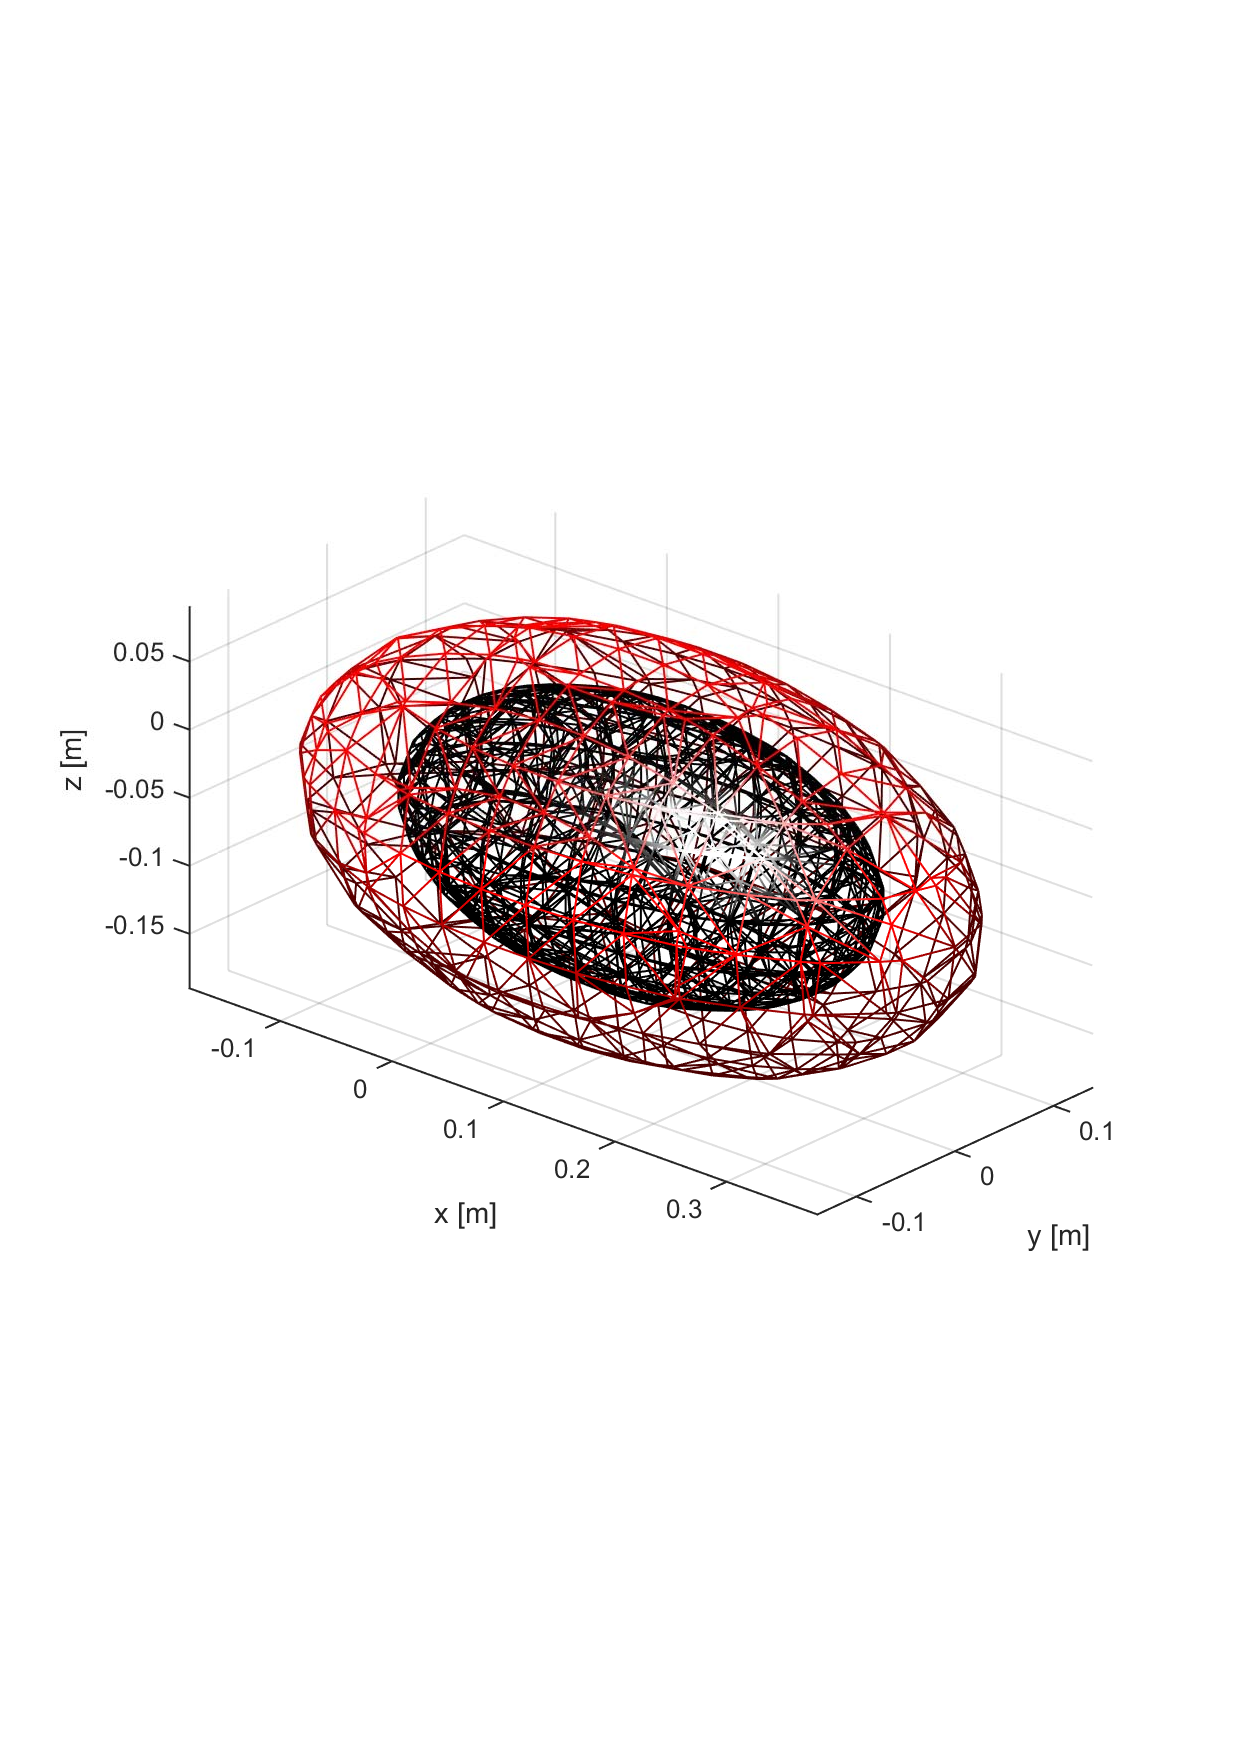
\includegraphics[width=0.7\textwidth]{zerolevelset_3d.pdf}
	\caption{Red marks the zero level set (and black marks the one level set, indicating that the ellipsoid encloses the region $\mathcal{X}_u$).}
	\label{fig:zerolevelset_3d}
\end{figure}

The third constraint in \autoref{def:barrier_certificate} is tested for a barrier certificate of this form with the system in \autoref{eq:3D_sys_static}. This is done by splitting the constraint up into the combined constraints on $L_gB(x)$ and $L_fB(x)$ from \autoref{req2}:
\begin{align}
L_gB_0(x) = \frac{dB_0(x,y,z)}{dx,y,z}g(x) &= 
\begin{bmatrix} 
\frac{2}{r_x^2}(c_x-x) & \frac{2}{r_y^2}(c_y-y) & \frac{2}{r_z^2}(c_z-z) 
\end{bmatrix}
\begin{bmatrix}
1/\tau& 0 & 0 \\ 0& 1/\tau & 0 \\0& 0& 1/\tau
\end{bmatrix} \nonumber\\
&= \frac{2}{\tau}
\begin{bmatrix} 
\frac{1}{r_x^2}(c_x-x) & \frac{1}{r_y^2}(c_y-y) & \frac{1}{r_z^2}(c_z-z) 
\end{bmatrix}
\end{align}
It can be seen that $L_gB(x)=0$ in the center of the ellipsoid $[c_x,c_y,c_z]$, and hence it is tested that $L_fB(x)<0$ in this point:
\begin{align}
L_fB_0(x) &= \frac{dB_0(x,y,z)}{dx,y,z}f(x) = 
\begin{bmatrix} 
\frac{2}{r_x^2}(c_x-x) & \frac{2}{r_y^2}(c_y-y) & \frac{2}{r_z^2}(c_z-z) 
\end{bmatrix}
\begin{bmatrix}
-1/\tau& 0 & 0 \\ 0& -1/\tau & 0 \\0& 0& -1/\tau
\end{bmatrix} 
\begin{bmatrix}
x\\y\\z
\end{bmatrix}\nonumber\\
& \phantom{=\frac{dB_0(x,y,z)}{dx,y,z}f(x)} =
-\frac{2}{\tau} \left(
\frac{1}{r_x^2}(c_xx-x^2) +\frac{1}{r_y^2}(c_yy-y^2) + \frac{1}{r_z^2}(c_zz-z^2) \right)\\
L_fB_0(c_x,c_y,c_z)&= 0 \nonumber
\end{align}
As this is the vertex of the barrier function, the relaxed requirement $L_fB(x)\leq 0$ applies, and hence this candidate barrier function is used in the design of the safety controller.

\textcolor{red}{pick the same values for K and N as before? Get measures for a heart to define the radii! Where should we define the center of the ellipsoid - should be such that the tool can reach all the way around it (but not necessarily below)}



THIS IS ONLY POSITION, NOT ORIENTATION

\subsection{Design of the CBF}
\textcolor{red}{design according to Allg\" ower and pick a value for epsilon (start of transition area)}

\section{Safe Controller Design for Second Order System}